\chapter{Methodology}
\label{ch:methodology}

The purpose of this work is to categorize medical words according to whether they can be understood or not by non-specialized people, using features obtained with deep learning methods. The manual annotations of these words described in the previous chapter provide the reference data. 

% The categorization pipeline is the following: after features for each word are computed, they are used for training the classifiers, and the results are evaluated using the cross-validation.

The proposed method includes three steps: 
\begin{enumerate}
    \item calculation of NLP features associated with the annotated words;
    \item training a machine learning model for words classification;
    \item evaluation of classification quality using cross-validation.
\end{enumerate}

In this research we want to provide answers to the following questions:
\begin{enumerate}
    \item Which feature set distinguishes better between understandable and non-understandable medical words?
    \item Why one feature set categorizes better than another?
    \item Do classifiers built on the considered feature sets generalize well? 
\end{enumerate}


\section{Feature sets}
\subsection{Standard NLP features}
\label{sec:standard-features}
We will refer to the previously used NLP features described in \citep{Grabar-PITR2014} as \textit{"standard features"} (opposed to two kinds of \textit{"embeddings"} described in the next subsection). They include 24 linguistic and extra-linguistic features related to general and specialized languages. The features are computed automatically and can be grouped into ten classes: 


\todo[inline]{In the list below, you should not use ``we'' to be
  honest since these you received the data with the NLP features. When
  reading the (false) impression that you compute the NLP features.}

\begin{itemize}
\item {\it Syntactic categories.}  Syntactic categories and lemmas are
  computed by TreeTagger \citep{Schmid-1994} and then checked
  \todo{th: corrected} by Flemm
  \citep{Namer-TAL2000}.  The syntactic categories are assigned to
  words within the context of their terms.  If a given word receives
  more than one category, the most frequent one is kept as feature.
  Among the main categories we find for instance nouns, adjectives,
  proper names, verbs and abbreviations.
\item {\it Presence of words in reference lexica.} We exploit two
  reference lexica of the French language:
  TLFi\footnote{\url{http://www.atilf.fr/}} and {\it lexique.org}\footnote{\url{http://www.lexique.org/}}. TLFi is
  a dictionary of the French language covering XIX and XX
  centuries. It contains almost 100,000 entries. {\it lexique.org} is
  a lexicon created for psycholinguistic experiments. It contains over
  135,000 entries, among which inflectional forms of verbs, adjectives
  and nouns. It contains almost 35,000 lemmas.
\item {\it Frequency of words through a non specialized search
    engine.} For each word, we query the Google search engine in order
  to know its frequency attested on the web.
\item {\it Frequency of words in the medical terminology.} We also
  compute the frequency of words in the medical terminology Snomed
  International.
\item {\it Number and types of semantic categories associated to
    words.} We exploit the information on the semantic categories of
  Snomed International.
\item {\it Length of words in number of their characters and
    syllables.} For each word, we compute the number of its characters
  and syllables.
\item {\it Number of bases and affixes.} Each lemma is analyzed by the
  morphological analyzer D\'erif \citep{Namer-AMIA2004}, adapted to the
  treatment of medical words. It performs the decomposition of lemmas
  into bases and affixes known in its database and it provides also
  semantic explanation of the analyzed lexemes. We exploit the
  morphological decomposition information (number of affixes and
  bases).
\item {\it Initial and final substrings of the words.}  We compute the
  initial and final substrings of different length, from three to five
  characters.
\item {\it Number and percentage of consonants, vowels and other
    characters.} We compute the number and the percentage of
  consonants, vowels and other characters (i.e., hyphen, apostrophe,
  comas).
\item {\it Classical readability scores.} We apply two classical
  readability measures: Flesch \citep{Flesch1948} and its variant
  Flesch-Kincaid \citep{Kincaid-1975}. Such measures are typically used
  for evaluating the difficulty level of a text. They exploit surface
  characteristics of words (number of characters and/or syllables) and
  normalize these values with specifically designed coefficients.
\end{itemize}
%%

\subsection{FastText word embeddings usage}

FastText word embeddings \cite{Bojanowski-ACL2017} is a good candidate as features for words difficulty detection task because they are able to use words' morphological information and generalize over it. The fact that word embeddings capture context and morphological information leads to the hypothesis that incorporating this information as features will improve classification accuracy for our specific problem. FastText embedding vectors are the sum of character n-gram representations, so that they could be generated even for unknown words. As we found out, being trained on Wikipedia and Common Crawl\footnote{\url{http://commoncrawl.org/}} texts the portion of known words from our dataset for current FastText embeddings is quite big. According to our analysis, 44.26\% (13,118 out of 29,641) medical words in the dataset and 56.00\% (16,598 out of 29,641) lowercased medical words in the dataset were used for training of the currently published FastText\footnote{\url{https://fasttext.cc}} model for French.

\subsection{French RNN Medical Understandability Text Embeddings (FrnnMUTE)}
\label{sec:frnnmute-learning}

According to the general functionality of RNN expressed in \ref{sec:rnn}, the final hidden state aggregates the information about all input sequence. This idea is frequently used to receive hidden representations of sequences. Sequence-to-sequence (seq2seq) models is a well-known example of how this idea works on practice \citep{Sutskever-NIPS2014}. Such models consist of two parts: an \textit{encoder} is an RNN which encodes input sequence into a representation in hidden space (which is also called \textit{thought vector}), and a \textit{decoder} which generates a new sequence out of the hidden representations (fig. \ref{fig:seq2seq}). 

\begin{figure}[h]
    \centering
    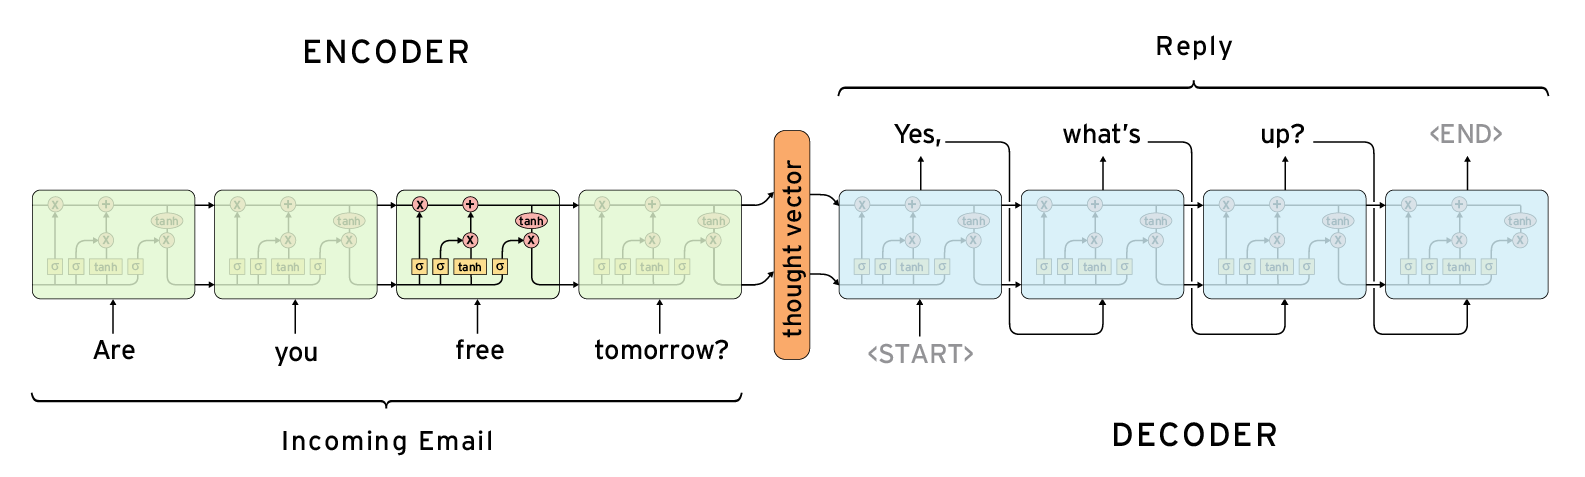
\includegraphics[width=14cm]{Images/seq2seq.png}
    \caption{A seq2seq model for question answering task. Source: \citep{Britz-2016}}
    \label{fig:seq2seq}
\end{figure} 

We utilized this idea for representing words from our dataset. To receive word representations from an RNN, we first trained it to classify words based on labels by one annotator (we chose $O1$), then for each word we found values of the last hidden state of the RNN and used this vector as features in words understandability detection for different users.

As a direct classifier, we trained a character-level RNN using PyTorch framework\footnote{\url{https://pytorch.org/}} and one GPU Tesla K80. For training we lowercased all words, converted them to a singular form and substituted all Unicode symbols with ASCII analogs.  We tried several RNN architectures and hyperparameter sets; the detailed information is available in Appendix \ref{appx:rnn}. 


The best F1-weighted on three classes we got for the following setting:

\begin{lstlisting}[language=Python]
{
'test_size': 0.1
'model': RNN(
  (lstm): LSTM(input_size=57, hidden_size=50, num_layers=2,
               dropout=0.7, bidirectional=False)
  (fc): Linear(in_features=50, out_features=3, bias=True))
}
\end{lstlisting}

\todo[inline]{Don't expect that everybody understand the code
  above. So you should not put code in the text (at least here), but
  explain the parameter values (test\_size, input\_size, etc.) and the
  configuration (what is LSTM ? FC ?). You never mention LSTM before.}


This model reached the best performance on the eighth epoch \todo{you
  must explain what is a epoch and maybe the impact on the results and
  the system} with $F1= 78.94$ and $accuracy =
81.21\%$\todo{Is the evaluation performed with development set or with
cross-validation?}. Using this model we received 50-dimensional words' representations which we called FrnnMUTE (French RNN Medical Understandability Text Embeddings). 


\section{Cross-validation scenarios}
For a thorough study of generalization abilities of the developed in this work classification models, we propose to consider three distinct cross-validation scenarios based on different combinations of users and vocabulary in train and test sets (fig. \ref{fig:experiments-description}).

\begin{figure}[h]
    \centering
    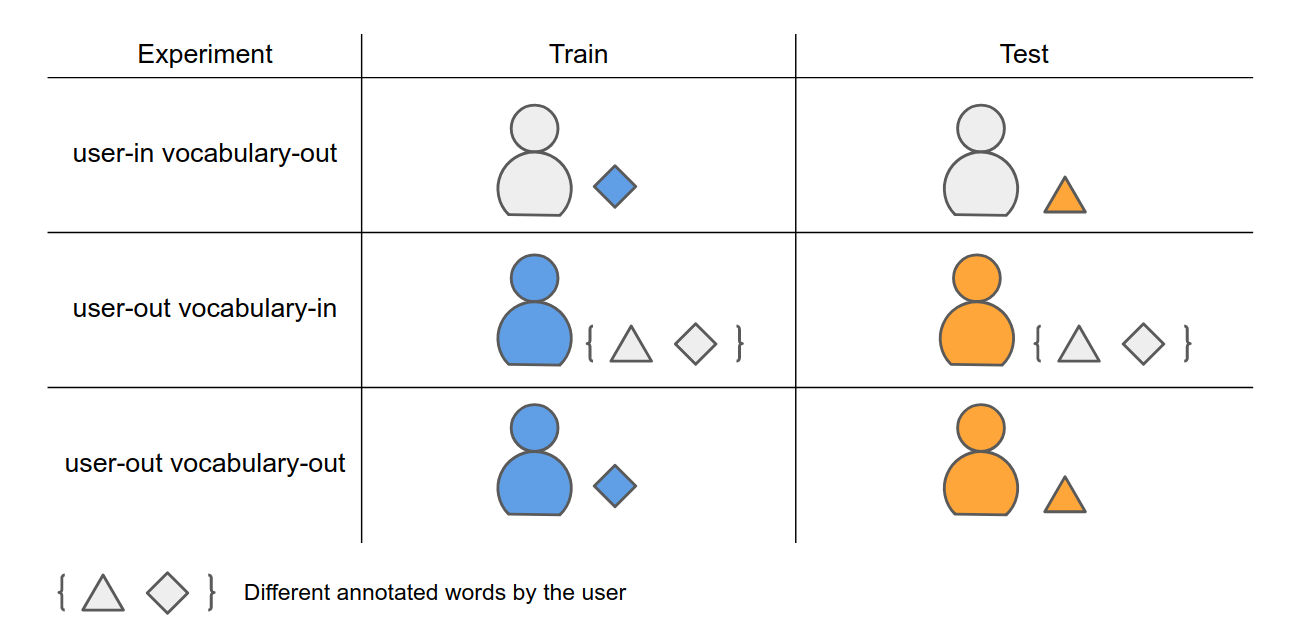
\includegraphics[width=14cm]{Images/Experiments.png}
    \caption{Visual description of experiments.}
    \label{fig:experiments-description}
\end{figure} 

\begin{enumerate}
    \item \textbf{User-in vocabulary-out cross-validation.} This type of experiment follows the scenario from the paper \citep{Grabar-PITR2014} we compare the results with throughout this work.  The cross-validation is done on each dataset (i.e., each user's annotation) separately. The goal of these experiments is to measure the ability of the method (classification model) to generalize class recognition on the \textit{known user} and his known manner to annotate words (that is, his understanding of the meaning of medical words) for \textit{unknown words}. 

\todo[inline]{In a pratical perspective: You may introduce the fact that user-in correspond to
  learning the profile of a user. So the model is a representation of
  the understanding/knowledge of the annotator.}
      
    \item \textbf{User-out vocabulary-in cross-validation.} In this experiment, we learn from all the annotations of one user and then test the model on annotations of another user. Thereby, in such a setting, we measure the ability of the classifier to generalize on all known words, but for unknown users. This scenario is realistic to a real-world situation: the reference annotations can be obtained only from a couple of users, presumably representing the overall population, but not from all the possible users. Yet, it is necessary to predict the familiarity of medical words for all the potential users even if they did not participate in the annotations.

\todo[inline]{similarly here, you can go further: The model represents the profile of a
  user/annotator and you try to identify if a new user has the same
  profile as a another. In that respect, for a user, the model that
  matches may be used to identify not understandable words for the new
user.}
      
    \item \textbf{User-out vocabulary-out cross-validation.} In this experiment, we take (k-1) folds of data from one user for training and use k-th fold for testing from the remaining user. In this case, we measure the ability of the method to generalize both on \textit{unknown users} and \textit{ unknown vocabulary}.

\todo[inline]{I think (but I'm not quite sure) that this last experiment must give you an idea of how many
  words you need to determine whether the profile of a user is the
  same as another.}
\end{enumerate}

\todo[inline]{You should add a conclusion or a discussion}